\documentclass{article}
\usepackage[UKenglish]{babel}
\usepackage[UKenglish]{isodate}
\usepackage{listings}
\usepackage{fullpage}
\usepackage{graphicx}
\usepackage{amsmath}
\usepackage{amsfonts}
\usepackage{amsthm}
\usepackage{subcaption}
\usepackage{mathtools}
\usepackage[vlined,ruled]{algorithm2e}
\usepackage[backend=bibtex, url=true]{biblatex}
\usepackage{tikz}

\bibliography{report.bib}
\theoremstyle{definition}
\newtheorem{definition}{Definition}
\SetKwProg{Function}{Function}{}{}
\SetKwFunction{expand}{expand}
\SetKwFunction{colouringBound}{colouringBound}
\SetKwFunction{cbIndSet}{colouringBoundForIndependentSet}
\author{Paulius Dilkas}
\title{Clique-Based Encodings for Graph Edit Distance}

\begin{document}
\maketitle
\begin{abstract}
  Graph edit distance (GED) is a common way to quantify the similarity between two graphs. We propose two ways to encode it into a clique-based problem with additional constraints (with weighted vertices and edges and with weighted vertices only). We model and compare the two encodings with a model based on the original definition of the problem using constraint programming. We propose a new branch-and-bound algorithm with a novel heuristic based on one of the encodings, evaluate its performance on public datasets, and compare our results with experimental results for state-of-the-art exact GED algorithms. We conclude by listing several improvements that are yet to be explored.
\end{abstract}
\section{Introduction}
Comparing how similar two objects are is an important task in Pattern Recognition. Although it is common to represent objects as vectors, encoding them as graphs can be advantageous. For instance, graphs allow for a more natural encoding of relationship information between different subparts (relative position, distance, etc.). The problem of conceptualising similarity between two graphs is called graph matching (GM) and it has two main branches: exact and error-tolerant. While exact methods solve problems such as (sub)graph isomorphism and maximum common subgraph, error-tolerant GM allows to directly match graphs that are not isomorphic to each other and provides a number, identifying how good the matching is. One such approach is called graph edit distance (GED) and is defined in Section \ref{sec:2}.
\section{Problem definition and proposed solutions}
\label{sec:2}
In this section we introduce all the ideas and definitions used in this paper. Section \ref{sec:ged} introduces the definition of graph edit distance. Section \ref{sec:cp} defines a constraint programming (CP) model corresponding to the main definition of the problem, which acts both as a way to check our understanding of the problem and as a baseline to compare other models to. Section \ref{sec:clique} introduces two clique-based GED encodings together with CP models for them. Finally, Section \ref{sec:alg} explains the proposed algorithm.
\subsection{The definition of graph edit distance}
\label{sec:ged}
\begin{definition}
  An \emph{attributed graph} $G = (V, E, L_V, L_E, \mu, \zeta)$ is a 6-tuple where:
  \begin{itemize}
  \item $V$ is a set of vertices,
  \item $E \subseteq V \times V$ is a set of edges,
  \item $L_V$ is a set of vertex attributes,
  \item $L_E$ is a set of edge attributes,
  \item $\mu : V \to L_V$ is a vertex labelling function,
  \item $\zeta : E \to L_E$ is an edge labelling function.
  \end{itemize}
\end{definition}
\begin{definition}
  A function $f: V_1 \cup \{ \epsilon \} \to V_2 \cup \{ \epsilon \}$ is an \emph{error-tolerant graph matching} from $G_1 = (V_1, E_1, L_{V_1}, L_{E_1}, \mu_1, \zeta_1)$ to $G_2 = (V_2, E_2, L_{V_2}, L_{E_2}, \mu_2, \zeta_2)$ where $\epsilon$ refers to the empty vertex if
  \begin{enumerate}
  \item considering only non-empty vertices, $f: V_1 \to V_2$ is bijective,
  \item $\forall u_1, u_2 \in V_1, f(u_1) \ne \epsilon \implies f(u_1) \ne f(u_2)$,
  \item $\forall v_1, v_2 \in V_2, f^{-1}(v_1) \ne \epsilon \implies f^{-1}(v_1) \ne f^{-1}(v_2)$.
  \end{enumerate}
\end{definition}
\begin{definition}
  Let $f: V_1 \to V_2$ be an error-tolerant GM between graphs $G_1 = (V_1, E_1)$ and $G_2 = (V_2, E_2)$ and let $c: (V_1 \cup \{ \epsilon \} \times V_2 \cup \{ \epsilon \}) \cup (E_1 \cup \{ \epsilon \} \times E_2 \cup \{ \epsilon \}) \to \mathbb{R}$ be an arbitrary cost function. The \emph{matching cost function} of $f$ is defined as
  \[
  \begin{aligned}
    c(f) &= \overbrace{\sum_{\substack{u_i \in V_1\\ f(u_i) \in V_2}} c(u_i, f(u_i))}^{\mathclap{\text{vertex substitutions}}} + \overbrace{\sum_{\substack{u_i \in V_1\\ f(u_i) = \epsilon}} c(u_i, \epsilon)}^{\mathclap{\text{vertex deletions}}} + \overbrace{\sum_{\substack{v_k \in V_2\\ f^{-1}(v_k) = \epsilon}} c(\epsilon, v_k)}^{\mathclap{\text{vertex insertions}}} \\
    &+ \overbrace{\sum_{\substack{e(u_i, u_j) \in E_1\\ e(f(u_i), f(u_j)) \in E_2}} c(e(u_i, u_j), e(f(u_i), f(u_j)))}^{\mathclap{\text{edge substitutions}}} + \overbrace{\sum_{\substack{e(u_i, u_j) \in E_1\\ e(f(u_i), f(u_j)) = \epsilon}} c(e(u_i, u_j), \epsilon)}^{\mathclap{\text{edge deletions}}} \\
    &+ \overbrace{\sum_{\substack{e(v_k, v_l) \in E_2\\ e(f^{-1}(v_k), f^{-1}(v_l)) = \epsilon}} c(\epsilon, e(v_k, v_l))}^{\mathclap{\text{edge insertions}}}.
  \end{aligned}
  \]
\end{definition}
\begin{definition}
  A \emph{graph edit operation} for an attributed graph $G = (V, E, L_V, L_E, \mu, \zeta)$ is one of the following:
  \begin{itemize}
  \item vertex insertion ($V' = V \cup \{ u_i \}$ for $u_i \not \in V$),
  \item vertex deletion ($V' = V \setminus \{ u_i \}$ for $u_i \in V$),
  \item vertex substitution (redefine $\mu$ so that $\mu(u_i) = l_i$),
  \item edge insertion ($E' = E \cup \{ e(u_i, u_j) \}$ for $e(u_i, u_j) \not \in E$, $u_i, u_j \in V$),
  \item edge deletion ($E' = E \setminus \{ e(u_i, u_j) \}$ for $e(u_i, u_j) \in E$).
  \end{itemize}
\end{definition}
\begin{definition}
  A set $\{ ed_1, \dots, ed_k \}$ of $k$ edit operations $ed_i$ that transform a graph $G_1$ completely into another graph $G_2$ is called a \emph{(complete) edit path} $\lambda(G_1, G_2)$ between $G_1$ and $G_2$. A partial edit path refers to a subset of $\{ ed_1, \dots, ed_k \}$. The set of all complete edit paths is denoted $\gamma(G_1, G_2)$.
\end{definition}
\begin{figure}
  \begin{subfigure}[t]{0.25\textwidth}
    \centering
    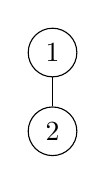
\begin{tikzpicture}
      \begin{scope}[every node/.style={circle,draw}]
        \node (a1) {1};
        \node (a2) [below of=a1] {2};
      \end{scope}
      \path (a1) edge node {} (a2);
    \end{tikzpicture}
    \caption{}
  \end{subfigure}
  \begin{subfigure}[t]{0.25\textwidth}
    \centering
    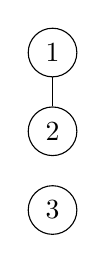
\begin{tikzpicture}
      \begin{scope}[every node/.style={circle,draw},xshift=4 cm]
        \node (b1) {1};
        \node (b2) [below of=b1] {2};
        \node (b3) [below of=b2] {3};
      \end{scope}
      \path (b1) edge node {} (b2);
    \end{tikzpicture}
    \caption{}
  \end{subfigure}
  \caption{One possible way to edit graph (a) into (b) is by inserting vertex 3 and matching everything else}
  \label{fig:example}
\end{figure}
For example, consider the graphs in Figure \ref{fig:example}. Then
\begin{equation}
\{ u_1 \to v_1, u_2 \to v_2, \epsilon \to v_3, e(u_1, u_2) \to e(v_1, v_2) \} \label{eqn:1} \tag{$\star$}
\end{equation}
is a complete edit path from (a) to (b). Note that instead of matching vertices this way, we could have matched them in 5 other ways or chosen to delete vertices/edges from (a) and insert the same number of vertices/edges to (b). Also note that it might be tempting to assume that a substitution is always cheaper than the sum of a deletion and an insertion, but that need not be the case. We will use this example (with the same edit path) in Section \ref{sec:clique} to illustrate how the same problem can be modeled in different ways.
\begin{definition}
  Let $G_1 = (V_1, E_1, L_{V_1}, L_{E_1}, \mu_1, \zeta_1)$ and $G_2 = (V_2, E_2, L_{V_2}, L_{E_2}, \mu_2, \zeta_2)$ be two attributed graphs and let $c$ be the cost function. The \emph{graph edit distance} between $G_1$ and $G_2$ is defined as
  \[ d_{\lambda_{\text{min}}}(G_1, G_2) = \min_{\lambda \in \gamma(G_1, G_2)} \sum_{ed_i \in \lambda} c(ed_i).\]
\end{definition}
\subsection{A constraint programming model}
\label{sec:cp}
To check if our definition of the problem is the same as in the literature and to compare our answers with a baseline solution, a simple CP model was implemented in MiniZinc.
\begin{lstlisting}
include "globals.mzn";

int: n1;
int: n2;
array[1..n1,1..n1] of 0..1: adjacent1;
array[1..n2,1..n2] of 0..1: adjacent2;
array[1..n2] of float: vertexInsertionCost;
array[1..n1,0..n2] of float: vertexSubstitutionCost;
array[1..n1,1..n1] of float: edgeDeletionCost;
array[1..n2,1..n2] of float: edgeInsertionCost;
array[1..n1,1..n1,1..n2,1..n2] of float: edgeSubstitutionCost;

array[1..n1] of var 0..n2: map; % 0 means deleted
array[1..n2] of var 0..n1: inverseMap; % 0 means inserted
var float: distance;

constraint alldifferent_except_0(map);
constraint alldifferent_except_0(inverseMap);
constraint forall(i in 1..n1 where map[i] != 0)(inverseMap[map[i]] == i);
constraint forall(j in 1..n2 where inverseMap[j] != 0)(
    map[inverseMap[j]] == j);
constraint distance == sum(i in 1..n1)(vertexSubstitutionCost[i,map[i]])
    + sum(j in 1..n2)(if inverseMap[j] == 0 then vertexInsertionCost[j]
        else 0 endif)
    + sum(i in 1..n1, j in 1..i-1 where adjacent1[i,j] == 1)(
        if map[i] == 0 \/ map[j] == 0 \/ adjacent2[map[i],map[j]] == 0
        then edgeDeletionCost[i,j]
        else edgeSubstitutionCost[i,j,map[i],map[j]] endif)
    + sum(i in 1..n2, j in 1..i-1 where adjacent2[i,j] == 1)(
        if inverseMap[i] == 0 \/ inverseMap[j] == 0 \/
        adjacent1[inverseMap[i],inverseMap[j]] == 0
        then edgeInsertionCost[i,j] else 0 endif);

solve minimize distance;
\end{lstlisting}
For a graph edit distance problem from $G_1 = (V_1, E_1, L_{V_1}, L_{E_1}, \mu_1, \zeta_1)$ to $G_2 = (V_2, E_2, L_{V_2}, L_{E_2}, \mu_2, \zeta_2)$, $\texttt{n1} = |V_1|$, $\texttt{n2} = |V_2|$, \texttt{adjacent1} and \texttt{adjacent2} are the adjacency matrices of graphs $G_1$ and $G_2$ respectively, and the rest of the data encodes parts of the cost function $c$. Vertex deletion cost is in the 0th column of \texttt{vertexSubstitutionCost}. Unfortunately, due to inaccuracies in working with floating-point numbers and/or bugs in gecode, this model fails on some problem instances with non-integer costs.
\subsection{Clique Encodings}
\label{sec:clique}
% TODO: write an introduction
\subsubsection{Putting weights on both vertices and edges}
\begin{figure}
  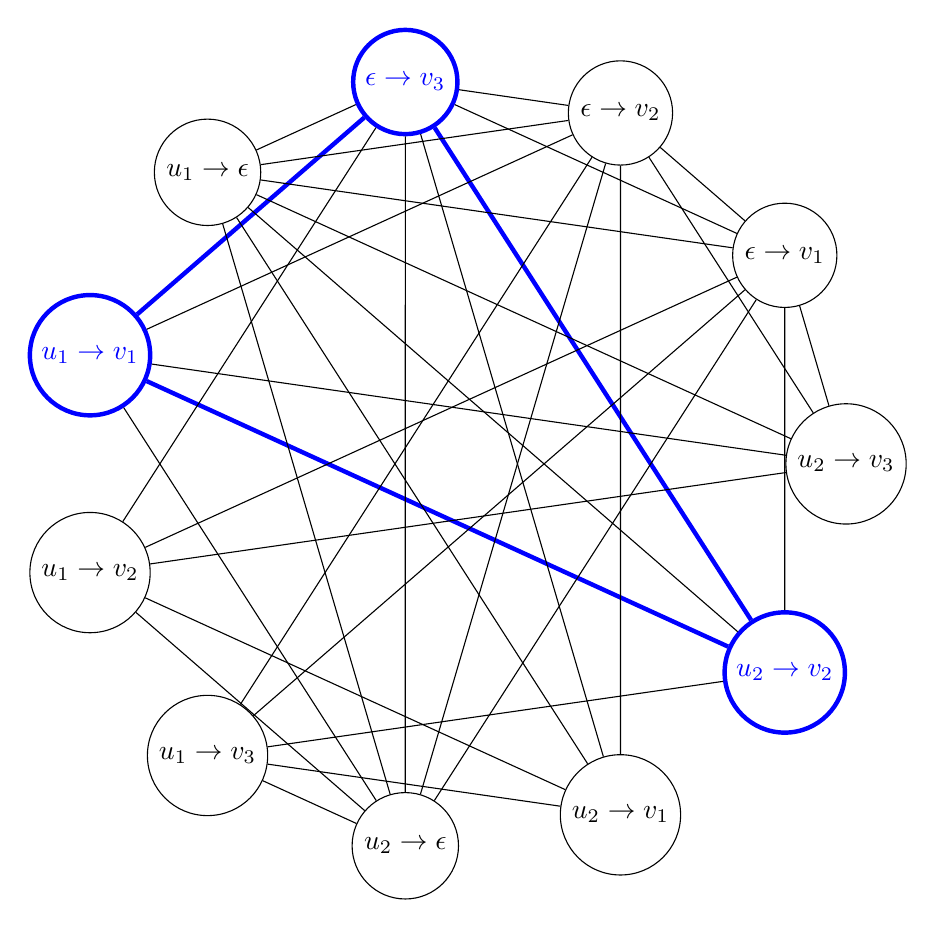
\begin{tikzpicture}[scale=0.7]
    \begin{scope}[every node/.style={circle,draw}]
      \node (i1) at (360/11 * 1:7cm) {$\epsilon \to v_1$};
      \node (i2) at (360/11 * 2:7cm) {$\epsilon \to v_2$};
      \node (i3) [color=blue,ultra thick] at (360/11 * 3:7cm) {$\epsilon \to v_3$};

      \node (d1) at (360/11 * 4:7cm) {$u_1 \to \epsilon$};
      \node (s11) [color=blue,ultra thick] at (360/11 * 5:7cm) {$u_1 \to v_1$};
      \node (s12) at (360/11 * 6:7cm) {$u_1 \to v_2$};
      \node (s13) at (360/11 * 7:7cm) {$u_1 \to v_3$};

      \node (d2) at (360/11 * 8:7cm) {$u_2 \to \epsilon$};
      \node (s21) at (360/11 * 9:7cm) {$u_2 \to v_1$};
      \node (s22) [color=blue,ultra thick] at (360/11 * 10:7cm) {$u_2 \to v_2$};
      \node (s23) at (360:7cm) {$u_2 \to v_3$};
    \end{scope}

    \begin{scope}[color=blue]
      \path (s11) [ultra thick] edge node {} (s22) edge node {} (i3);
      \path (s22) [ultra thick] edge node {} (i3);
    \end{scope}

    \path (i1) edge node {} (i2) edge node {} (i3) edge node {} (d1) edge node {} (s12) edge node {} (s13) edge node {} (d2) edge node {} (s22) edge node {} (s23);
    \path (i2) edge node {} (i3) edge node {} (d1) edge node {} (s11) edge node {} (s13) edge node {} (d2) edge node {} (s21) edge node {} (s23);
    \path (i3) edge node {} (d1) edge node {} (s12) edge node {} (d2) edge node {} (s21);
    \path (d1) edge node {} (d2) edge node {} (s21) edge node {} (s22) edge node {} (s23);
    \path (s11) edge node {} (d2) edge node {} (s23);
    \path (s12) edge node {} (d2) edge node {} (s21) edge node {} (s23);
    \path (s13) edge node {} (d2) edge node {} (s21) edge node {} (s22);
  \end{tikzpicture}
  \caption{Vertex-edge-weights encoding of the example from Figure \ref{fig:example} with the clique corresponding to the edit path \ref{eqn:1} in blue}
  \label{fig:encoding1}
\end{figure}
Let $G_1 = (V_1, E_1, L_{V_1}, L_{E_1}, \mu_1, \zeta_1)$ and $G_2 = (V_2, E_2, L_{V_2}, L_{E_2}, \mu_2, \zeta_2)$ be two arbitrary attributed graphs and let $c: (V_1 \cup \{ \epsilon \} \times V_2 \cup \{ \epsilon \}) \cup (E_1 \cup \{ \epsilon \} \times E_2 \cup \{ \epsilon \}) \to \mathbb{R}$ be an arbitrary cost function. Assume that $c(\epsilon, \epsilon) = 0$, $e(v_i, \epsilon) = e(\epsilon, v_i) = e(\epsilon, \epsilon) = \epsilon$ for all $v_i \in V_1 \cup V_2$, and $e(v_i, v_j) = \epsilon$ if there is no edge between $v_i$ and $v_j$. We will construct a new graph such that finding a minimum weight clique on it would be equivalent to finding the graph edit distance between $G_1$ and $G_2$. Construct a new weighted graph $G_3 = (V_3, E_3, L_{V_3} \subseteq \mathbb{R}, L_{E_3} \subseteq \mathbb{R}, \mu_3, \zeta_3)$ such that:
\begin{itemize}
\item $V_3$ has a 1-to-1 correspondence with the set of all possible edit operations on vertices: $\{ \epsilon \to v_i : v_i \in V_2 \} \cup \{ v_i \to v_j : v_i \in V_1, v_j \in V_2 \} \cup \{ v_i \to \epsilon : v_i \in V_1 \}$,
\item there is an edge between two vertices if and only if they don't share a common vertex in $V_1$ or $V_2$,
\item for an arbitrary vertex edit operation $v_i \to v_j$ (with $v_i \in V_1 \cup \{ \epsilon \}, v_j \in V_2 \cup \{ \epsilon \}$) corresponding to $v \in V_3$, $\mu_3(v) = c(v_i, v_j)$,
\item for an edge $\phi$ between vertices corresponding to edit operations $v_i \to v_j$, $v_k \to v_l$ (where $v_i, v_k \in V_1 \cup \{ \epsilon \}$, $v_j, v_l \in V_2 \cup \{ \epsilon \}$),
  \[
  \zeta_3(\phi) = \begin{cases}
    \min(c(e(v_i, v_k), e(v_j, v_l)), c(e(v_i, v_k), \epsilon) + c(\epsilon, e(v_j, v_l))), & \text{if } e(v_i, v_k) \in E_1, e(v_j, v_l) \in E_2, \\
    c(e(v_i, v_k), e(v_j, v_l)) & \text{otherwise.}
  \end{cases}
  \]
\end{itemize}

All operations on edges of $G_1$ and $G_2$ are encoded into edges in $G_3$, hence we only need to choose operations on vertices (represented by vertices of $G_3$) and operations on edges can be inferred from edges of $G_3$ that are part of the clique. Figure \ref{fig:encoding1} shows the resulting $G_3$ for graphs from Figure \ref{fig:example}.

Furthermore, we must make sure that exactly one edit operation is performed on each vertex. Having multiple edit operations per vertex is already impossible because vertices of $G_3$, representing operations that have vertices of $G_1$ or $G_2$ in common, are not adjacent in $G_3$ by definition. Enforcing the need to pick an operation for each vertex of $G_1$ and $G_2$ requires new constraints, easily encoded in this CP model (which in the following sections will be referred to as the vertex-edge-weights model):
\begin{lstlisting}
include "globals.mzn";

int: v1;
int: v2;
int: n = (v1+1)*(v2+1)-1; % number of vertices
array[1..n] of float: vertexWeights;
array[1..n,1..n] of float: edgeWeights;
array[1..n,1..n] of 0..1: adjacent; % adjacency matrix
array[1..n] of var 0..1: clique; % whether a vertex is part of the clique
var float: distance;

% clique property
constraint forall(i in 1..n, j in 1..i-1)(
    adjacent[i,j] == 0 -> clique[i] + clique[j] <= 1);
% we must pick a vertex from each independent set
constraint forall(i in 1..v1)(sum(j in 0..v2)(clique[i*(v2+1)+j]) >= 1);
constraint forall(j in 1..v2)(sum(i in 0..v1)(clique[i*(v2+1)+j]) >= 1);
constraint distance == sum(i in 1..n)(clique[i] * vertexWeights[i])
    + sum(i in 1..n, j in 1..i-1)(clique[i] * clique[j] * edgeWeights[i,j]);

solve minimize distance;
\end{lstlisting}
\subsubsection{Weights on vertices only}
\begin{figure}
  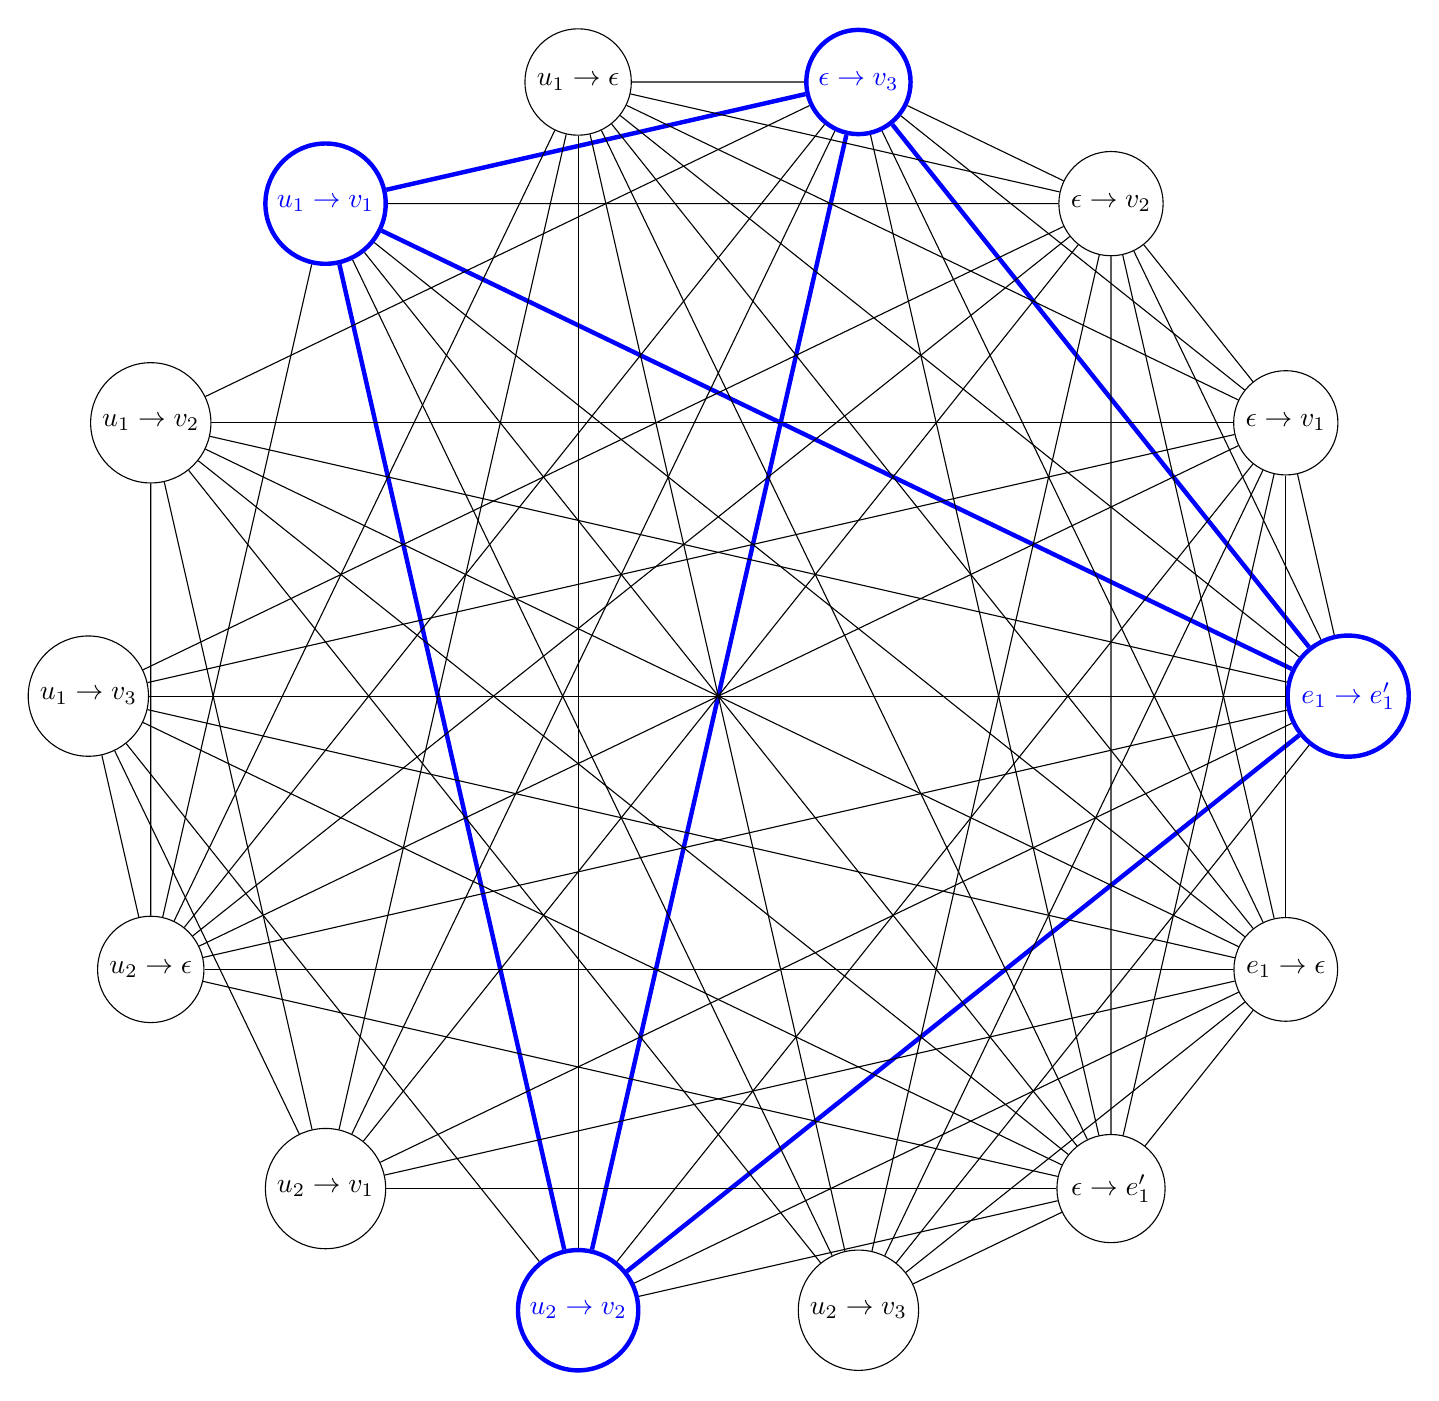
\begin{tikzpicture}
    \begin{scope}[every node/.style={circle,draw}]
      \node (vi1) at (360/14 * 1:8cm) {$\epsilon \to v_1$};
      \node (vi2) at (360/14 * 2:8cm) {$\epsilon \to v_2$};
      \node (vi3) [color=blue,ultra thick] at (360/14 * 3:8cm) {$\epsilon \to v_3$};

      \node (vd1) at (720/7:8cm) {$u_1 \to \epsilon$};
      \node (vs11) [color=blue,ultra thick] at ({720/7 + 360/14 * 1}:8cm) {$u_1 \to v_1$};
      \node (vs12) at ({720/7 + 360/14 * 2}:8cm) {$u_1 \to v_2$};
      \node (vs13) at ({720/7 + 360/14 * 3}:8cm) {$u_1 \to v_3$};

      \node (vd2) at (720/7 + 360/14 * 4:8cm) {$u_2 \to \epsilon$};
      \node (vs21) at ({720/7 + 360/14 * 4 + 360/14 * 1}:8cm) {$u_2 \to v_1$};
      \node (vs22) [color=blue,ultra thick] at ({720/7 + 360/14 * 4 + 360/14 * 2}:8cm) {$u_2 \to v_2$};
      \node (vs23) at ({720/7 + 360/14 * 4 + 360/14 * 3}:8cm) {$u_2 \to v_3$};

      \node (ei) at (2160/7:8cm) {$\epsilon \to e_1'$};
      \node (ed) at (2340/7:8cm) {$e_1 \to \epsilon$};
      \node (es) [color=blue,ultra thick] at (360:8cm) {$e_1 \to e_1'$};
    \end{scope}

    \begin{scope}[draw=blue]
      \path (vi3) [ultra thick] edge node {} (vs11) edge node {} (vs22) edge node {} (es);
      \path (vs11) [ultra thick] edge node {} (vs22) edge node {} (es);
      \path (vs22) [ultra thick] edge node {} (es);
    \end{scope}

    \path (vi1) edge node {} (vi2) edge node {} (vi3) edge node {} (vd1) edge node {} (vs12) edge node {} (vs13) edge node {} (vd2) edge node {} (vs22) edge node {} (vs23) edge node {} (ei) edge node {} (ed) edge node {} (es);
    \path (vi2) edge node {} (vi3) edge node {} (vd1) edge node {} (vs11) edge node {} (vs13) edge node {} (vd2) edge node {} (vs21) edge node {} (vs23) edge node {} (ei) edge node {} (ed) edge node {} (es);
    \path (vi3) edge node {} (vd1) edge node {} (vs12) edge node {} (vd2) edge node {} (vs21) edge node {} (ei) edge node {} (ed);
    \path (vd1) edge node {} (vd2) edge node {} (vs21) edge node {} (vs22) edge node {} (vs23) edge node {} (ei) edge node {} (ed) edge node {} (es);
    \path (vs11) edge node {} (vd2) edge node {} (vs23) edge node {} (ei) edge node {} (ed);
    \path (vs12) edge node {} (vd2) edge node {} (vs21) edge node {} (vs23) edge node {} (ei) edge node {} (ed) edge node {} (es);
    \path (vs13) edge node {} (vd2) edge node {} (vs21) edge node {} (vs22) edge node {} (ei) edge node {} (ed) edge node {} (es);
    \path (vd2) edge node {} (ei) edge node {} (ed) edge node {} (es);
    \path (vs21) edge node {} (ei) edge node {} (ed) edge node {} (es);
    \path (vs22) edge node {} (ei) edge node {} (ed);
    \path (vs23) edge node {} (ei) edge node {} (ed) edge node {} (es);
    \path (ei) edge node {} (ed);
  \end{tikzpicture}
  \caption{Vertex-weights encoding of the example from Figure \ref{fig:example} with the clique corresponding to the edit path \ref{eqn:1} in blue}
  \label{fig:encoding2}
\end{figure}
Let $G_1 = (V_1, E_1, L_{V_1}, L_{E_1}, \mu_1, \zeta_1)$ and $G_2 = (V_2, E_2, L_{V_2}, L_{E_2}, \mu_2, \zeta_2)$ be two arbitrarily attributed graphs. Create a new graph $G_3 = (V_3, E_3, L_{V_3} \subseteq \mathbb{R}, \emptyset, \mu_3)$ with weights on vertices and no edge labels defined as follows:
\begin{itemize}
\item $V_3$ has a 1-to-1 correspondence with the set of all possible edit operations $\{ \epsilon \to v_i : v_i \in V_2 \} \cup \{ v_i \to v_j : v_i \in V_1, v_j \in V_2 \} \cup \{ v_i \to \epsilon : v_i \in V_1 \} \cup \{ \epsilon \to e_i : e_i \in E_2 \} \cup \{ e_i \to e_j : e_i \in E_1, e_j \in E_2 \} \cup \{ e_i \to \epsilon : e_i \in E_1 \}$.
\item  $E_3$ can be defined in terms of what edges it does not contain:
  \begin{itemize}
  \item Similarly to the previous encoding, for all $v_i, v_k \in V_1 \cup E_1 \cup \{ \epsilon \}, v_j, v_l \in V_2 \cup E_2 \cup \{ \epsilon \}$, there is no edge between vertices in $G_3$ representing $v_i \to v_j$ and $v_k \to v_l$ if and only if $v_i = v_k \ne \epsilon$ or $v_j = v_l \ne \epsilon$.
  \item For all $v_i \in V_1 \cup \{ \epsilon \}, v_j \in V_2 \cup \{ \epsilon \}, e(v_k, v_l) \in E_1, e(v_m, v_n) \in E_2$, there is no edge between vertices in $G_3$ representing $v_i \to v_j$ (any edit operation on vertices) and $e(v_k, v_l) \to e(v_m, v_n)$ (edge substitution) if:
    \begin{itemize}
    \item $v_i = \epsilon$ and $v_j \in \{ v_m, v_n \}$ (edge substitution is not compatible with insertion of an incident vertex),
    \item $v_j = \epsilon$ and $v_i \in \{ v_k, v_l \}$ (same for vertex deletion),
    \item $v_i, v_j \ne \epsilon$ and ($v_i \in \{ v_k, v_l \}$ and $v_j \not \in \{ v_m, v_n \}$ or $v_j \in \{ v_m, v_n \}$ and $v_i \not \in \{ v_k, v_l \}$) (vertex substitution $v_i \to v_j$ is compatible with an edge substitution if and only if both $v_i$ and $v_j$ are mentioned in the edge substitution or neither).
    \end{itemize}
    NB: there is always an edge between any edge insertion/deletion and any edit operation on vertices.
  \end{itemize}
\item Define $L_{V_3}$ and $\mu_3: V_3 \to L_{V_3}$ so that if $v_i \in V_3$ corresponds to any edit operation $ed_i$ from $G_1$ to $G_2$, then $\mu_3(v_i) = c(ed_i)$.
\end{itemize}
Then finding a minimum weight clique in $G_3$ is equivalent to finding the graph edit distance between $G_1$ and $G_2$, provided we add two new constraints to the MiniZinc model, ensuring that all edges in $E_1 \cup E_2$ have some edit operation associated with them. We will refer to this new model as the vertex-weights model. Figure \ref{fig:encoding2} illustrates this encoding for graphs from Figure \ref{fig:example} with $e(u_1, u_2)$ and $e(v_1, v_2)$ denoted as $e_1$ and $e_1'$, respectively.
\begin{lstlisting}
include "globals.mzn";

int: v1;
int: e1;
int: v2;
int: e2;
int: n = v1+v2+e1+e2+v1*v2+e1*e2; % number of vertices
int: e0 = (v1+1)*(v2+1) - 1; % index of the last vertex operation
array[1..n] of float: weights;
array[1..n,1..n] of 0..1: adjacent; % adjacency matrix
array[1..n] of var 0..1: clique; % whether a vertex is part of the clique
var float: distance;

% clique property
constraint forall(i in 1..n, j in 1..i-1)(
    adjacent[i,j] == 0 -> clique[i]+clique[j] <= 1);
% we must pick a vertex from each independent set
constraint forall(i in 1..v1)(sum(j in 0..v2)(clique[i*(v2+1)+j]) >= 1);
constraint forall(j in 1..v2)(sum(i in 0..v1)(clique[i*(v2+1)+j]) >= 1);
constraint forall(i in 1..e1)(sum(j in 0..e2)(clique[e0+i*(e2+1)+j]) >= 1);
constraint forall(j in 1..e2)(sum(i in 0..e1)(clique[e0+i*(e2+1)+j]) >= 1);
constraint distance == sum(i in 1..n)(clique[i] * weights[i]);

solve minimize distance;
\end{lstlisting}
\subsection{The proposed algorithm}
\label{sec:alg}
In order to use one of these clique encodings for any speed benefits, a state-of-the-art algorithm known as BITCLIQUE \cite{tavares_2016} (with its heuristic function called BITCOLOR, also known as Tavares' colouring) for solving maximum weight clique was adapted for the vertex-weights model. To find the graph edit distance between two attributed graphs $G_1 = (V_1, E_1, L_{V_1}, L_{E_1}, \mu_1, \zeta_1), G_2 = (V_2, E_2, L_{V_2}, L_{E_2}, \mu_2, \zeta_2)$, we create a new weighted graph $G = (V, E, L_V, \emptyset, \mu)$ according to the vertex-weights model, fix an order on $V_1 \cup V_2 \cup E_1 \cup E_2$, and construct a sequence of sets $(S_i)_{i=0}^{|V_1|+|V_2|+|E_1|+|E_2|-1}$, where $S_i \subset V$ is a set of all vertices corresponding to edit operations on the ith element of $V_1 \cup V_2 \cup E_1 \cup E_2$. These sets correspond to the additional constraints of the MiniZinc model. The resulting search algorithm is described in Algorithm \ref{alg:1} and the new heuristic function is described in Algorithm \ref{alg:2}.
\begin{algorithm}
  \KwIn{The number of vertices in the graph $n$, an adjacency matrix expressed as an array of bitsets \textit{adjacencyBitsets}, a weight function $w: \{0, 1, ..., n-1\} \to \mathbb{R}^+$, a sequence of sets $(S_i)_{i=0}^{k-1}$}
  \KwOut{A sequence of vertices $(v_j)_{j=1}^k$ comprising a clique in the graph such that for each set $S_i \in (S_i)_{i=0}^{k-1}$, there is a vertex $v_j \in (v_j)_{j=1}^k$ such that $v_j \in S_i$}
  bitset $P \gets \underbrace{1\dots1}_{\mathclap{n}}$\;
  initialise empty lists $C$, \textit{incumbent}\;
  $\mathtt{expand}(\mathit{adjacencyBitsets}, w, (S_i)_{i=0}^{k-1}, C, P, \mathit{incumbent})$\;
  \Return{\textit{incumbent}}\;
  \Function{\expand{$\mathit{adjacencyBitsets}, w, (S_i)_{i=0}^{k-1}, C, P, \mathit{incumbent}$}}{
    initialise a 2-dimensional array \textit{cumulativeWtBound} with $k$ rows and $|S_i|$ columns for $0 \le i < k$\;
    $\mathit{indSet} \gets \mathtt{colouringBound}(w, (S_i)_{i=0}^{k-1}, P, C, \mathit{cumulativeWtBound})$\;
    \If{$\mathit{indSet} = \mathit{IMPOSSIBLE\_TO\_SATISFY}$}{
      \Return\;
    }
    \If{$\mathit{indSet} = \mathit{ALL\_CONSTRAINTS\_SATISFIED}$}{
      \If{$|\mathit{incumbent}| = 0$ or $\sum_{v \in C} w(v) < \sum_{v \in \mathit{incumbent}} w(v)$}{
        $\mathit{incumbent} \gets C$\;
      }
      \Return\;
    }
    \For{$v \in \{i : 0 \le i < |S_{\mathit{indSet}}|$, $P[S_{\mathit{indSet},i}] = 1\}$ in the order of ascending $\mathit{cumulativeWtBound}[\mathit{indSet},v]$}{
      $C.\mathtt{push}(S_{\mathit{indSet},v})$\;
      $\mathtt{expand}(\mathit{adjacencyBitsets}, w, (S_i)_{i=0}^{k-1}, C, P \cap \mathit{adjacencyBitsets}[S_{\mathit{indSet},v}], \mathit{incumbent})$\;
      $C.\mathtt{pop}()$\;
    }
  }
  \caption{The main algorithm with a recursive search function}
  \label{alg:1}
\end{algorithm}
\begin{algorithm}
  \Function{\colouringBound{$w, (S_i)_{i=0}^{k-1}, P, C, \mathit{cumulativeWtBound}$}}{
    $\mathit{bound} \gets 0$\;
    $\mathit{smallestIndependentSet} \gets 0$\;
    $\mathit{minVerticesInP} \gets \infty$\;
    $\mathit{independentSetSatisfied} = [\underbrace{0, 0, \dots 0}_{\mathclap{k}}]$\;
    $\mathit{residualWt} \gets [w(v) : 0 \le v < n]$\;
    \tcc{Choose the independent set with the smallest number of members in $P$ to explore first}
    \For{$i \gets 0, \dots, k-1$}{
      $\mathit{howManyVerticesInP} \gets 0$\;
      \For{$v \in S_i$}{
        \If{$v \in C$}{
          $\mathit{independentSetSatisfied}[i] = 1$\;
          \KwSty{break}\;
        }
        \If{$P[v] = 1$}{
          $\mathit{howManyVerticesInP} \gets \mathit{howManyVerticesInP} + 1$\;
        }
      }
      \If{$\mathit{independentSetSatisfied}[i] = 0$}{
        \If{$\mathit{howManyVerticesInP} == 0$}{
          \Return \textit{IMPOSSIBLE\_TO\_SATISFY}\;
        }
        \If{$\mathit{howManyVerticesInP} < \mathit{minVerticesInP}$}{
          $\mathit{smallestIndependentSet} \gets i$\;
          $\mathit{minVerticesInP} \gets \mathit{howManyVerticesInP}$\;
        }
      }
    }
    \If{$\mathit{minVerticesInP} = \infty$}{
      \Return \textit{ALL\_CONSTRAINTS\_SATISFIED}\;
    }
    \For{$i \gets 0, \dots, k-1$}{
      \If{($\mathit{independentSetSatisfied}[i] = 0$) and $i \ne \mathit{smallestIndependentSet}$}{
        $\mathtt{colouringBoundForIndependentSet}(i, \mathit{residualWt}, \mathit{bound}, P, \mathit{cumulativeWtBound})$\;
      }
    }
    $\mathtt{colouringBoundForIndependentSet}(\mathit{smallestIndependentSet}, \mathit{residualWt}, \mathit{bound}, P,$\\
    \qquad $\mathit{cumulativeWtBound})$;
  }
  \Function{\cbIndSet{$i, \mathit{residualWt}, \mathit{bound}, P, \mathit{cumulativeWtBound}$}}{
    $\mathit{classMinWt} \gets \min\{\mathit{residualWt}[v] : v \in S_i, P[v] = 1\}$\;
    \For{$j \gets 0, \dots, |S_i|-1$}{
      $\mathit{residualWt}[S_{i,j}] \gets \mathit{residualWt}[S_{i,j}] - \mathit{classMinWt}$\;
      $\mathit{cumulativeWtBound}[i,j] \gets \mathit{bound} + \mathit{residualWt}[S_{i,j}]$\;
    }
  }
  \caption{Tavares' colouring adapted to produce lower bounds for GED}
  \label{alg:2}
\end{algorithm}
\section{Implementation and evaluation}
\subsection{Data and its formatting}
GDR4GED \cite{abu-aisheh_raveaux_ramel_2015}, a graph data repository for graph edit distance, was chosen to be used for algorithm evaluation and comparison. It contains four databases: GREC, MUTA, Protein, and CMU, with graph sizes ranging from 5 to 70 vertices. It also has ground truth values for some of the pairs of graphs, stating the optimal graph edit distance and a way to achieve it. To describe instances of this vertex-weights clique encoding, DIMACS format was extended in several ways:
\begin{itemize}
\item The first line now reads: \texttt{p edge n m v1 v2 e1 e2}, where:
  \begin{itemize}
  \item \texttt{n} and \texttt{m} are the numbers of vertices and edges in the encoding graph, respectively (as usual),
  \item \texttt{v1} and \texttt{v2} are the numbers of vertices in the original graphs,
  \item \texttt{e1} and \texttt{e2} are the numbers of edges in the original graphs.
  \end{itemize}
  The primary reason for this addition is that $\texttt{v1}+\texttt{v2}+\texttt{e1}+\texttt{e2}$ is the number of independent sets that our model must pick a vertex from. Moreover, having all four numbers instead of just their sum allows us to recover information about which vertex represents which operation, which is not used by our main algorithm, but could be useful in deciding which independent set should be picked from first (variable ordering), which vertex is picked to satisfy the independent set (value ordering), or in considering different heuristic functions.
  \item Along with \texttt{e} indicating edges and \texttt{n} indicating vertex weights, we add lines starting with \texttt{s} indicating independent sets. Each such line is a space-separated list of vertex numbers (ranging from 1 to \texttt{n}), where we are required to pick one of them to be in the clique (picking more than one is always impossible since they form an independent set).
\end{itemize}
\subsection{Evaluation}
\begin{figure}
  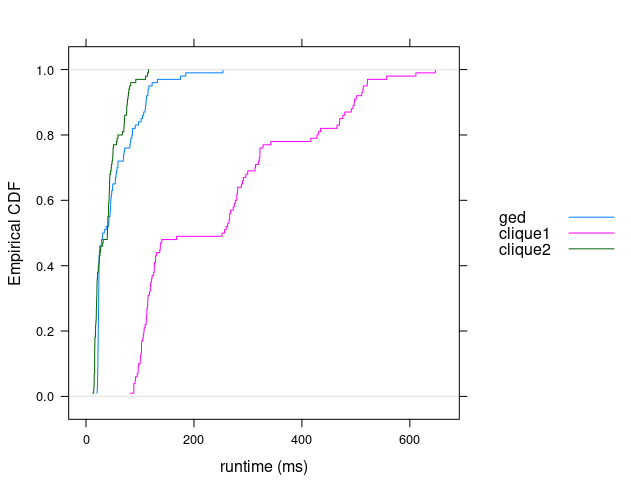
\includegraphics[scale=0.75]{comparison.png}
  \caption{Comparing running times of all 3 models}
  \label{fig:comparison}
\end{figure}
We begin by comparing the three MiniZinc models and plotting their cumulative (ECDF) plots in Figure \ref{fig:comparison}, which shows the vertex-edge-weights model to be significantly inferior to the other two. The initial CP model and the vertex-weights encoding are about equal, with the latter eventually outperforming the former.

Our new algorithm (with its heuristic function) was implemented in C and proved to be orders of magnitude faster, finishing these 5-vertex GED problem instances with a maximum running time of 1 ms. Therefore, to evaluate it, we ran the algorithm with a 15 s time limit on GDR4GED datasets of appropriate sizes, namely: GRECMIX, GREC15, MUTA20, and Protein20. According to Figure \ref{fig:ecdf}, most problem instances are either very easy or very hard. The easy instances are usually the ones that have a very small optimal distance.
\begin{figure}
  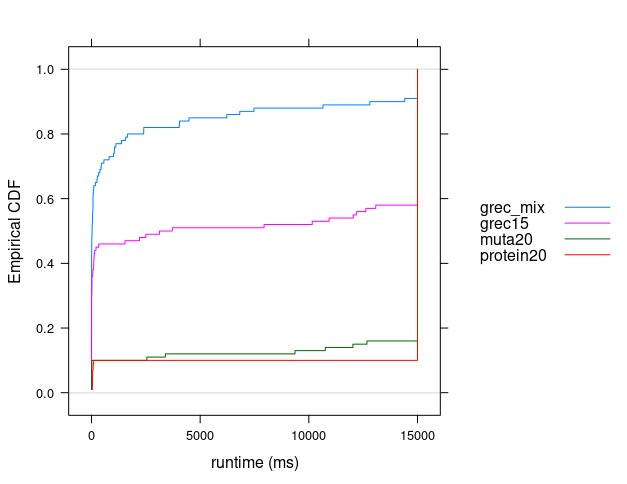
\includegraphics[scale=0.75]{ecdfs.png}
  \caption{ECDF plots on various datasets with a 15 s time limit}
  \label{fig:ecdf}
\end{figure}
\section{Discussion and related work}
To compare our solution with other algorithms that are solving the same problem, we are only considering algorithms in the literature that are both exact and sequential. However, one approximate algorithm deserves special attention as it is the most widely used heuristic for many exact GED algorithms \cite{abu-aisheh_raveaux_ramel_martineau_2015}, including the ones reviewed in this section. The algorithm is known as the bipartite (BP) heuristic and works by reformulating graph matching as an assignment problem and solving it by using Munkres' algorithm \cite{riesen_bunke_2009}. There are two algorithms that we would like to highlight:
\begin{itemize}
\item A widely used algorithm for solving GED is based on A* search \cite{riesen_fankhauser_bunke_2011}. However, it suffers from high memory consumption \cite{abu-aisheh_raveaux_ramel_martineau_2015}.
\item The state-of-the-art sequential algorithm for GED seems to be DF-GED \cite{abu-aisheh_raveaux_ramel_martineau_2015}, a branch-and-bound search algorithm.
\end{itemize}

Although we were not able to make direct comparisons by running these algorithms on the same machine, the hardware described in \cite{abu-aisheh_raveaux_ramel_martineau_2015} is equivalent to the hardware used for our experiments. Thus, comparing our results on several GREC datasets, we can recognise that:
\begin{itemize}
\item DF-GED is able to find the optimal answer in 350 ms in all of the data (but not necessarily proves it to be correct), while Algorithm \ref{alg:1} has non-zero deviations (as defined in \cite{abu-aisheh_raveaux_ramel_martineau_2015}) with a maximum of 0.05 with a 15 s time limit even on GREC15.
\item A* fails to finish in 350 ms with most of GREC10 data, while Algorithm \ref{alg:1} successfully finishes with a mean running time of 34.73 ms and a maximum running time of 195 ms.
\end{itemize}
\section{Conclusions and future work}
Although the proposed algorithm did not outperform DF-GED, some important ideas were left untouched:
\begin{itemize}
\item Adapting the same algorithm to work with the vertex-edge-weights model. This might make the heuristic function less precise, but will result in less recursive function calls and handling quadratically less data.
\item Exploring other heuristic functions, such as the aforementioned BP heuristic or one of its later variants.
\item What vertex we choose to add to the clique at every node of the search tree can significantly affect the algorithm's performance. This is done in two stages:
  \begin{enumerate}
  \item First we choose which independent set to pick from. We choose the set with the smallest number of vertices that can still be added to the clique.
  \item Then we order vertices in the selected independent set by their lower bounds and start with the smallest lower bound.
  \end{enumerate}
  Although these choices seem reasonable, perhaps there are better alternatives that should be explored.
\item Creating a parallel version of the algorithm.
\end{itemize}
\printbibliography
\end{document}
